\documentclass[conference]{IEEEtran}
\usepackage[utf8]{inputenc}
\usepackage{amsmath,amssymb,booktabs,graphicx,url,xcolor}
\usepackage[hidelinks]{hyperref}
\newcommand{\TOVERIFY}[1]{\textcolor{red}{[TO VERIFY: #1]}}
\graphicspath{{figures/}}

\begin{document}

\title{How Often Do Citation Verifiers Flag Genuine References?\\
A Controlled Comparison on Pre-LLM Bibliographies}

\author{\IEEEauthorblockN{Satyala Murali Karthik (MCL2026010)}
\IEEEauthorblockA{Department of Information Technology, IIIT Allahabad}}

\maketitle

% Abstract is written LAST (Prompt 15) so it matches the final evidence.
\begin{abstract}
Registry-based citation verifiers are usually evaluated on known fabrications, so their false-positive
rate (FPR) on genuine references is rarely measured. I score five matching rules---two from my
literature review (existence-only V1E and full-fidelity V1F), the published rules of Naser (V2) and
Neralla et al.\ (V3), and an author-veto ablation (V3a)---on one frozen set of Crossref, OpenAlex and arXiv
responses for 567 cited \texttt{.bib} entries from 19 pre-ChatGPT arXiv cs.CL papers and 807 fabricated
citations from desk-rejected ICLR~2026 submissions. Recall is 95.7--99.9\%, but FPR is 16.0--17.3\% for
V1E, V2 and V3 and 47.1\% for V1F. At a fabrication prevalence of 1\%, at most 5.7\% of flags would be
correct. About 86--89\% of the false positives of V1E, V2 and V3 occur because the cited paper is not
among the retrieved candidates; references carrying a DOI were never flagged by these three rules,
whereas 22\% of references with neither a DOI nor an arXiv ID were. The author veto changed no outcome.
Adjudicating every flagged reference of V1E, V2 and V3 against independent sources shows that about
85\% of their flags fall on references that are entirely correct (adjusted FPR 13.9--15.2\%). The results
come from one field and one quarter of arXiv submissions.
\end{abstract}

\begin{IEEEkeywords}
citation verification, hallucinated references, false positive rate, positive predictive value, scholarly metadata
\end{IEEEkeywords}

%======================================================================
\section{Introduction}
Large language models can produce bibliographic references that do not exist or that mix
fields from several real papers, a failure mode that follows from how such models are trained and
scored~\cite{kalai2025}. Registry-based verifiers answer by looking each citation up in
open scholarly registries (Crossref, arXiv, OpenAlex) and flagging those that cannot be matched.
Such tools are usually evaluated on collections of \emph{known} fabrications, which measures
recall. My literature review~\cite{karthik2026review} (\S5.1--5.2) identified that their
false-positive rate (FPR) on ordinary genuine reference lists is rarely reported; yet when only
0.5--5\% of citations are fabricated, the share of flags that are correct (positive predictive
value, PPV) is dominated by the FPR (review Eq.~13).

This paper measures that quantity directly. I score five published or derived matching rules on
one frozen set of registry responses for (i) cited \texttt{.bib} entries of arXiv cs.CL papers
submitted before the release of ChatGPT and (ii) 807 fabricated or badly wrong citations from
desk-rejected ICLR~2026 submissions released with CiteTracer~\cite{li2026citetracer,citetracerrepo}.

\textbf{Research questions.}
\textbf{RQ1:} What FPR do the verifiers have on genuine pre-LLM references?
\textbf{RQ2:} What PPV does this imply at prevalence $\pi \in \{0.5,1,2,5\}\%$?
\textbf{RQ3:} Which reference types and failed checks cause the false positives?

\textbf{Hypotheses} (fixed on 28 Oct 2026, before any result).
\textbf{H1:} V1F has a higher FPR than V1E, because it adds field checks on top of the existence test;
contradicted if the two differ by less than one point.
\textbf{H2:} No verifier reaches PPV $\ge 0.5$ at $\pi=1\%$, which would require FPR $\le$ recall$/99$;
contradicted by any verifier above that line.
\textbf{H3:} \texttt{misc}, \texttt{book}, \texttt{phdthesis} and arXiv-cited entries have the highest
FPR, because registries index them least consistently; contradicted if FPR is roughly equal across strata.

\textbf{Contribution.} The problem is not new~\cite{badalova2026,neralla2026}; the contribution is
a measurement: a controlled comparison under a single retrieval pass, prevalence-aware PPV, and
an error analysis of false positives. No new detector is proposed.


\textbf{Findings in brief.} All verifiers catch almost every fabricated citation, but they also flag
about one in six genuine references (V1F: almost one in two). At realistic prevalence this makes most flags
wrong. The false positives are mainly a retrieval problem: the dominant predictor is whether the
citation carries a persistent identifier, not which scoring rule is used.

%======================================================================
\section{Related Work}
\textbf{Detectors evaluated on fabrications.} CiteTracer~\cite{li2026citetracer} combines a cache,
scholarly connectors, a web agent and LLM judges, and reports catching 97.1\% of a real
fabricated set; its real set contains positives only. Neralla et al.~\cite{neralla2026} flag
94 of 100 NeurIPS~2025 fabrications (66 as ``likely hallucinated'', the rest as ``partial'') with a
weighted title/author/journal score against Semantic Scholar.
\textbf{Evaluations that include genuine references.} Badalova and Mayr~\cite{badalova2026} ran
five open tools on 104 references (71 verified, 33 problematic) from three documents; the tools
flagged 20--53 of the 71 verified references (their Table~4; FPR 28--75\% by my arithmetic). Their
sample is small and has no prevalence or threshold analysis.
\textbf{Scale of the problem.} Naser~\cite{naser2026} audits 69,557 LLM-generated citations
across 10 models using a title-Jaccard rule (re-used here as V2) and reports that 8 of 75
``hallucinated'' citations checked by hand were real. Zhao et al.~\cite{zhao2026} estimate
fabrication in the wild across 111\,M references, motivating pre-LLM bibliographies as a clean
reference point.

%======================================================================
\section{Method}
\subsection{Verifiers}
All verifiers receive a citation $c$ and the same candidate list $R(c)$ from the registries.
\begin{itemize}
\item \textbf{V1E} (existence; review Eq.~2): flag unless some candidate has
$0.7\,s_{\text{title}} + 0.3\,s_{\text{auth}} \ge 0.85$, with $s_{\text{title}}$ a normalised
Levenshtein similarity (Eq.~3) and $s_{\text{auth}}$ surname overlap.
\item \textbf{V1F} (fidelity; Eqs.~2--5, label Eq.~9): V1E plus title $\ge 0.90$, all cited
surnames present, exact year, venue similarity $\ge 0.5$, matching locators and identifiers.
\item \textbf{V2} (Naser~\cite{naser2026} \S3.4): $100(0.6\,J_{\text{title}} + 0.2\,a + 0.2\,y)$;
flag below 80.
\item \textbf{V3} (Neralla et al.~\cite{neralla2026} Eq.~1): $0.60\,t + 0.25\,a + 0.15\,j$ (fuzzy
title, authors, journal); flag below 80.
\item \textbf{V3a} (ablation): V3 with an author veto (author score $<50$ $\Rightarrow$ not
verified) and no substitution of the title score for missing authors.
\end{itemize}
V2 and V3 are re-implementations from the papers' text; V3's exact fuzzy function is not
stated in the paper and is not in the authors' repository (which holds evaluation notebooks
only; commit 7e7d019~\cite{nerallarepo}), so I use normalised Levenshtein$\times 100$. As in the
source, a citation is counted as flagged when $S<80$ (``partial'' or ``likely hallucinated'').

\subsection{Retrieval}
\begin{figure*}[t]
\centering
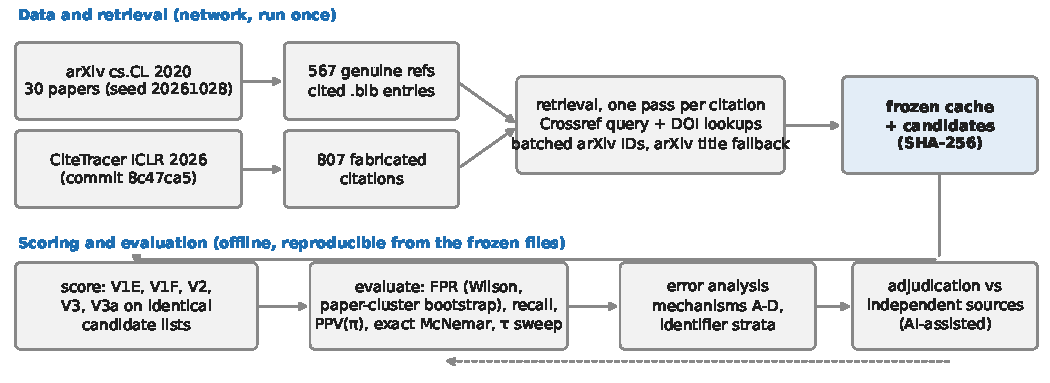
\includegraphics[width=0.96\textwidth]{pipeline.pdf}
\caption{Study pipeline. Retrieval runs once over the network; everything below the frozen,
checksummed cache is offline and reproducible. All five verifiers score identical candidate lists.}
\label{fig:pipeline}
\end{figure*}
One pass per citation (Fig.~\ref{fig:pipeline}): Crossref~\cite{crossrefapi} bibliographic query
(5 rows, polite pool); Crossref and OpenAlex~\cite{openalexapi} DOI lookups when a DOI is cited;
arXiv~\cite{arxivapi} ID lookups (batched, $\le$100 IDs per request); and an arXiv title search when
no candidate yet has title similarity $\ge 0.8$. Every response is cached in SQLite; the cache and
candidate file are frozen and hashed before scoring, so verifier differences come from scoring rules
alone.

\subsection{Metrics}
Primary: FPR on genuine references with Wilson 95\% intervals and a paper-level cluster bootstrap
(2,000 resamples), since references of one paper are correlated. Secondary: recall on the
fabricated set; PPV at prevalence $\pi$,
\[ \mathrm{PPV}(\pi) = \frac{\mathrm{TPR}\,\pi}{\mathrm{TPR}\,\pi + \mathrm{FPR}\,(1-\pi)} \]
(review Eq.~13), checked by bootstrap mixing. Verifiers are compared pairwise on the same genuine
references with an exact McNemar test; a difference counts only if $p<0.05$ \emph{and} the FPR gap
is at least 2 points (frozen decision rule).

%======================================================================
\section{Experimental Setup}
\textbf{Genuine set.} arXiv cs.CL papers submitted between 1 Jan 2020 and 29 Nov 2022 were
listed (first $4\times200$ results), and 30 were sampled with seed 20261028. Only \texttt{.bib}
entries that the paper's \texttt{.tex} actually cites were kept.
Of the 30 sampled papers, 19 shipped a \texttt{.bib} file and contributed 567 cited references
(\texttt{inproceedings} 368, \texttt{article} 172, other types 27); 58 carry a DOI and 88 an arXiv ID.

\textbf{Fabricated set.} 807 citations from 647 desk-rejected ICLR~2026 submissions
(CiteTracer repository, commit 8c47ca5). The paper reports 957; the repository ships 807.
\textbf{Leakage.} Citing papers cannot occur in both sets (2020 arXiv vs.\ 2026 ICLR); the
evaluation script audits ID prefixes, duplicate IDs and label/flag validity.
\textbf{Protocol.} Thresholds were fixed from the source papers on 28 Oct 2026
(\texttt{configs/protocol.json}) before any live result. Amendments made for time and measured
API limits (30 instead of 100 papers; OpenAlex title search disabled because the keyless budget
allows $\sim$100 searches/day; 30 adjudicated flags per verifier) were logged on 13 Nov 2026
before results were seen. Because the arXiv API repeatedly timed out, retrieval ran in two phases
(Crossref and identifier lookups first, then the arXiv title fallback) with the same final candidate
lists as a single pass; failed requests were retried rather than cached.
\textbf{Environment.} Windows 11 laptop, Python 3.12.10, requests 2.34.2, matplotlib 3.11.2;
CPU only, no GPU and no LLM calls.

\subsection{Baseline validation before the experiment}
No published numbers exist for these rules on these data, so ``validating the baseline'' means showing
that the scoring stage behaves as the source papers specify before it is pointed at real bibliographies.
Three checks were run, all before the live retrieval.

\emph{Unit tests.} 33 tests fix the behaviour of the similarity function, surname and identifier
normalisation, the Wilson interval, the exact McNemar test, review Eq.~13 (it reproduces the worked
example in the review, 0.246) and the frozen cache.

\emph{Oracle retrieval.} Each of CiteTracer's 2,450 synthetic citations was scored against its own seed
record as the only candidate, which removes retrieval from the picture and isolates scoring
(Table~\ref{tab:oracle}). Every verifier flags 0 of 1,023 real and 0 of 271 borderline citations
(95\% Wilson upper bound 0.4\%), so none of them is trigger-happy on clean metadata. The recall column
exposes properties of the published rules that matter later: V2 scores a year-only error at exactly 80,
its own ``confirmed'' threshold, so it catches none of H4; V3 scores a venue-only error at 85 and misses
all of H3; V1F misses 99 of 166 H6 cases because publisher and location lie outside review Eq.~4.

\emph{End-to-end run.} The full \texttt{score} $\rightarrow$ \texttt{evaluate} pipeline was executed on
those 2,450 citations and its audit passed. This run is a code check only and is never reported as a
result (decision D21): with perfect retrieval and clean seeds, the synthetic ``real'' class cannot
produce a false positive, which is precisely why the FPR question needs natural bibliographies.

\begin{table}[t]
\centering\footnotesize
\caption{Baseline validation: share flagged (\%) under oracle retrieval on CiteTracer's synthetic set.
Reproduced byte-for-byte on the laptop from the 28 Oct run.}
\label{tab:oracle}
\resizebox{\columnwidth}{!}{\begin{tabular}{lrrrrrr}
\toprule
Subtype & $n$ & V1E & V1F & V2 & V3 & V3a \\
\midrule
Real R1--R3 (false positives) & 1023 & 0.0 & 0.0 & 0.0 & 0.0 & 0.0 \\
Potential P1, P3 (false positives) & 271 & 0.0 & 0.0 & 0.0 & 0.0 & 0.0 \\
H1 title altered & 200 & 75.5 & 91.5 & 77.0 & 65.5 & 65.5 \\
H2 authors altered & 198 & 33.3 & 67.2 & 0.0 & 33.3 & 33.3 \\
H3 venue altered & 197 & 0.0 & 98.0 & 0.0 & 0.0 & 0.0 \\
H4 year altered & 195 & 0.0 & 100.0 & 0.0 & 0.0 & 0.0 \\
H5 DOI fabricated & 200 & 0.0 & 77.0 & 0.0 & 0.0 & 0.0 \\
H6 pages/volume/publisher/location & 166 & 0.0 & 40.4 & 0.0 & 0.0 & 0.0 \\
\midrule
All fabricated (recall) & 1156 & 18.8 & 80.0 & 13.3 & 17.0 & 17.0 \\
\bottomrule
\end{tabular}
}
\end{table}

\subsection{Reproducibility}
After retrieval the response cache and the candidate file were copied, hashed with SHA-256 and left
untouched (\texttt{results/frozen\_checksums.txt}). Everything from scoring onward reads only those
frozen files, so the central result regenerates offline in under a minute with two commands:
\begin{quote}\footnotesize\ttfamily
\noindent python scripts/score.py \\
\hspace*{1.5em}-{}-refs data/genuine\_refs.jsonl \\
\hspace*{3em}data/fabricated\_refs.jsonl \\
\hspace*{1.5em}-{}-candidates \\
\hspace*{3em}data/frozen/candidates\_20261113.jsonl \\[2pt]
\noindent python scripts/evaluate.py \\
\hspace*{1.5em}-{}-scores results/scores.csv \\
\hspace*{1.5em}-{}-adjudication \\
\hspace*{3em}results/adjudication\_sample.csv
\end{quote}
Re-running these reproduced \texttt{scores.csv} and \texttt{metrics.csv} byte-for-byte. Seeds are fixed
in \texttt{configs/protocol.json} (20261028 for paper sampling, bootstraps and the adjudication draw).
Two further scripts guard the manuscript itself: one re-derives every number quoted here from the result
files and fails on any disagreement, the other checks the \LaTeX{} structure. Raw data and the cache are
not redistributed (the positives' licence is unstated); the repository documents how to rebuild them.

\textbf{Code and data availability.} The repository contains the source, configurations, unit tests,
every result file and log, the decision and AI-assistance logs, and this manuscript:
\url{https://github.com/Karthik0069dev/AITR_Lab02_MCL2026010_CiteFPR}.

%======================================================================
\section{Results}
All numbers in this section are generated from \texttt{results/*.csv} by
\texttt{scripts/make\_tables.py}; retrieval completed for every citation (three passes, no request left
without a definitive answer), and the evaluation audit found no duplicate IDs, invalid labels or set
overlap.

\subsection{RQ1: false-positive rate}
\begin{table}[t]
\centering\footnotesize
\caption{FPR on 567 genuine references (top) and recall on 807 ICLR~2026 fabrications (bottom).
Paper-cluster CI: 2,000 bootstrap resamples of the 19 citing papers.}
\label{tab:fpr}
\resizebox{\columnwidth}{!}{\begin{tabular}{lrrrr}
\toprule
Verifier & FP / $n$ & FPR (\%) & 95\% Wilson & Paper-cluster CI \\
\midrule
V1E & 96 / 567 & 16.9 & [14.1, 20.2] & [12.2, 21.7] \\
V1F & 267 / 567 & 47.1 & [43.0, 51.2] & [38.7, 55.3] \\
V2 & 91 / 567 & 16.0 & [13.3, 19.3] & [11.9, 20.2] \\
V3 & 98 / 567 & 17.3 & [14.4, 20.6] & [12.6, 22.1] \\
V3a & 98 / 567 & 17.3 & [14.4, 20.6] & [12.6, 22.1] \\
\midrule
Verifier & \multicolumn{2}{r}{Recall (\%)} & \multicolumn{2}{r}{95\% Wilson} \\
\midrule
V1E & \multicolumn{2}{r}{99.1} & \multicolumn{2}{r}{[98.2, 99.6]} \\
V1F & \multicolumn{2}{r}{99.9} & \multicolumn{2}{r}{[99.3, 100.0]} \\
V2 & \multicolumn{2}{r}{95.7} & \multicolumn{2}{r}{[94.0, 96.9]} \\
V3 & \multicolumn{2}{r}{99.3} & \multicolumn{2}{r}{[98.4, 99.7]} \\
V3a & \multicolumn{2}{r}{99.3} & \multicolumn{2}{r}{[98.4, 99.7]} \\
\bottomrule
\end{tabular}
}
\end{table}

Table~\ref{tab:fpr} and Fig.~\ref{fig:fpr} show that V1E, V2 and V3 flag 16.0--17.3\% of genuine references
while recalling 95.7--99.3\% of fabrications. V1F flags 47.1\%.

\begin{figure}[t]
\centering
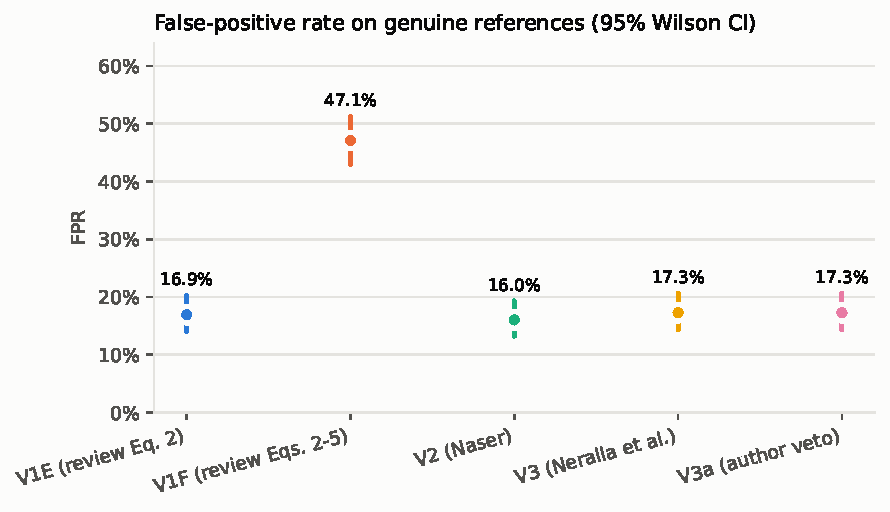
\includegraphics[width=\columnwidth]{fpr_by_verifier.pdf}
\caption{FPR on the 567 genuine references, with 95\% Wilson intervals.}
\label{fig:fpr}
\end{figure} The paper-cluster intervals are wider than the Wilson
intervals (e.g.\ V1E 12.2--21.7\% vs.\ 14.1--20.2\%), confirming that errors cluster by citing paper:
per-paper V1E FPR ranges from 0\% to 35\%.

Pairwise exact McNemar tests (Table~\ref{tab:mcnemar}) find that V1F differs from every other rule
(169--176 discordant pairs, all in one direction, $p<10^{-10}$, gap 29.8--31.0 points). Among V1E, V2 and
V3 no difference meets the frozen decision rule: the largest gap is 1.2 points (V2 vs.\ V3, $p=0.039$, below
the 2-point threshold). V3 and V3a produce identical flags on every genuine and fabricated citation.

\begin{table}[t]
\centering\footnotesize
\caption{Exact McNemar tests on genuine references. Rule met: $p<0.05$ and $|\text{gap}|\ge 2$ points.}
\label{tab:mcnemar}
\resizebox{\columnwidth}{!}{\begin{tabular}{lrrrrc}
\toprule
Pair & $a$ only & $b$ only & Gap (pts) & $p$ (exact) & Rule met \\
\midrule
V1E vs V1F & 0 & 171 & -30.2 & $<10^{-10}$ & yes \\
V1E vs V2 & 6 & 1 & +0.9 & 0.125 & no \\
V1E vs V3 & 0 & 2 & -0.4 & 0.5 & no \\
V1E vs V3a & 0 & 2 & -0.4 & 0.5 & no \\
V1F vs V2 & 176 & 0 & +31.0 & $<10^{-10}$ & yes \\
V1F vs V3 & 169 & 0 & +29.8 & $<10^{-10}$ & yes \\
V1F vs V3a & 169 & 0 & +29.8 & $<10^{-10}$ & yes \\
V2 vs V3 & 1 & 8 & -1.2 & 0.0391 & no \\
V2 vs V3a & 1 & 8 & -1.2 & 0.0391 & no \\
V3 vs V3a & 0 & 0 & +0.0 & 1 & no \\
\bottomrule
\end{tabular}
}
\end{table}

\subsection{RQ2: precision at realistic prevalence}
\begin{table}[t]
\centering\footnotesize
\caption{PPV from review Eq.~13 at fabrication prevalence $\pi$ (bootstrap-mixing values agree within 0.001).}
\label{tab:ppv}
\begin{tabular}{lrrrr}
\toprule
Verifier & $\pi=0.5\%$ & $\pi=1\%$ & $\pi=2\%$ & $\pi=5\%$ \\
\midrule
V1E & 0.029 & 0.056 & 0.107 & 0.236 \\
V1F & 0.011 & 0.021 & 0.042 & 0.100 \\
V2 & 0.029 & 0.057 & 0.108 & 0.239 \\
V3 & 0.028 & 0.055 & 0.105 & 0.232 \\
V3a & 0.028 & 0.055 & 0.105 & 0.232 \\
\bottomrule
\end{tabular}

\end{table}

Because FPR is large relative to $\pi$, PPV is low (Table~\ref{tab:ppv}, Fig.~\ref{fig:ppv}). At $\pi=1\%$,
5.5--5.7\% of flags from V1E, V2 or V3 are fabrications and 2.1\% for V1F; even at $\pi=5\%$ no rule exceeds
0.24. Reaching PPV $\ge 0.5$ at $\pi=1\%$ with recall near 1 would require FPR $\le 1\%$, about 16 times
lower than observed.

\begin{figure}[t]
\centering
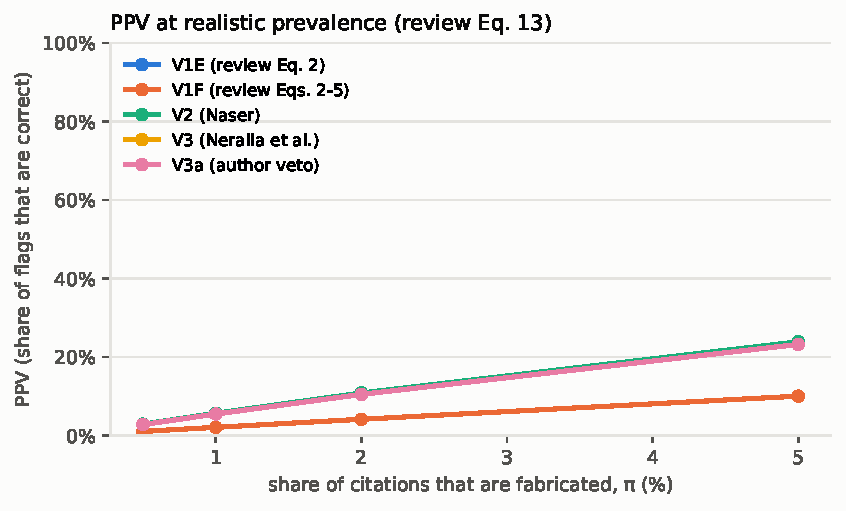
\includegraphics[width=\columnwidth]{ppv_by_prevalence.pdf}
\caption{PPV as a function of prevalence (review Eq.~13) for each verifier.}
\label{fig:ppv}
\end{figure}

\subsection{RQ3: causes of false positives}
\textbf{Retrieval vs.\ scoring.} I classified each false positive by its candidate list
(\texttt{scripts/fp\_mechanisms.py}): (A) no candidate with title similarity $\ge 0.8$; (B) a same-title
candidate whose authors disagree; (C) the right paper, rejected on year, venue, locator or score details;
(D) a near-miss title. Table~\ref{tab:mech} shows that for V1E, V2 and V3 the great majority of false
positives are type A: the cited paper never entered the candidate list. For V1F, 170 of its 267 are type C,
i.e.\ the correct record was found but a field disagreed.

\begin{table}[t]
\centering\footnotesize
\caption{False positives on genuine references by mechanism.}
\label{tab:mech}
\resizebox{\columnwidth}{!}{\begin{tabular}{lrrrrr}
\toprule
Verifier & FP & A: not retrieved & B: authors differ & C: field differs & D: near miss \\
\midrule
V1E & 96 & 84 & 7 & 1 & 4 \\
V1F & 267 & 84 & 7 & 170 & 6 \\
V2 & 91 & 81 & 4 & 1 & 5 \\
V3 & 98 & 84 & 7 & 2 & 5 \\
V3a & 98 & 84 & 7 & 2 & 5 \\
\bottomrule
\end{tabular}
}
\end{table}

\textbf{Identifiers.} No reference carrying a DOI ($n=58$) was flagged by V1E, V2 or V3; references with an
arXiv ID ($n=88$) were flagged at 1.1--3.4\%; those with neither ($n=423$) at 21.3--22.5\%
(Table~\ref{tab:ident}). For V1F the pattern reverses for arXiv-ID references (63.6\%), because the cited
conference venue and year rarely match the arXiv record.

\begin{table}[t]
\centering\footnotesize
\caption{FPR (\%) by the identifier the citation carries.}
\label{tab:ident}
\resizebox{\columnwidth}{!}{\begin{tabular}{lrrrrrr}
\toprule
Citation carries & $n$ & V1E & V1F & V2 & V3 & V3a \\
\midrule
a DOI & 58 & 0.0 & 12.1 & 0.0 & 0.0 & 0.0 \\
an arXiv ID & 88 & 3.4 & 63.6 & 1.1 & 3.4 & 3.4 \\
no identifier & 423 & 22.0 & 48.2 & 21.3 & 22.5 & 22.5 \\
\bottomrule
\end{tabular}
}
\end{table}

\textbf{Entry types.} \texttt{misc}, \texttt{book}, \texttt{techreport} and \texttt{incollection} entries are
flagged at 43--100\% by V1E, but each stratum has fewer than 30 references, so the frozen decision rule
(stratum FPR $\ge 2\times$ overall with $n\ge 30$) cannot be applied (Table~\ref{tab:type}).

\begin{table}[t]
\centering\footnotesize
\caption{FPR (\%) by BibTeX entry type.}
\label{tab:type}
\resizebox{\columnwidth}{!}{\begin{tabular}{lrrrrrr}
\toprule
Entry type & $n$ & V1E & V1F & V2 & V3 & V3a \\
\midrule
inproceedings & 368 & 15.8 & 40.0 & 14.9 & 16.0 & 16.0 \\
article & 172 & 12.8 & 55.8 & 11.6 & 13.4 & 13.4 \\
misc & 9 & 66.7 & 77.8 & 66.7 & 66.7 & 66.7 \\
incollection & 7 & 42.9 & 85.7 & 42.9 & 42.9 & 42.9 \\
book & 6 & 66.7 & 100.0 & 66.7 & 66.7 & 66.7 \\
techreport & 2 & 100.0 & 100.0 & 100.0 & 100.0 & 100.0 \\
phdthesis & 1 & 0.0 & 100.0 & 0.0 & 0.0 & 0.0 \\
inbook & 1 & 0.0 & 100.0 & 0.0 & 0.0 & 0.0 \\
online & 1 & 100.0 & 100.0 & 100.0 & 100.0 & 100.0 \\
\bottomrule
\end{tabular}
}
\end{table}

\textbf{Threshold sensitivity.} Lowering the thresholds removes few false positives
(Fig.~\ref{fig:tau}): at 60 instead of the published 80/85, FPR is still 13.2--14.6\% while recall drops
to 87--90\%. The false positives score low because the right record is absent, not because they sit near
the threshold.

\begin{figure}[t]
\centering
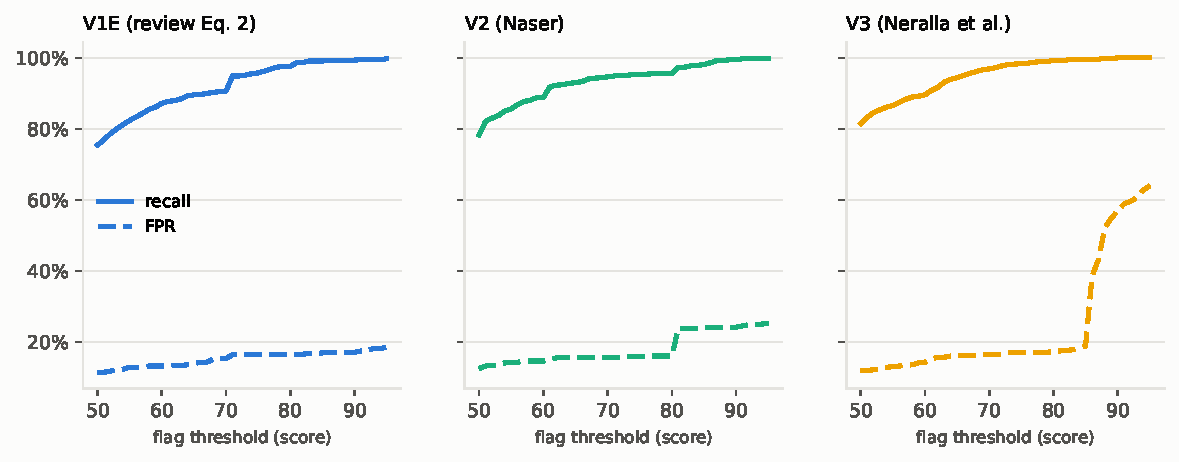
\includegraphics[width=\columnwidth]{tau_sweep.pdf}
\caption{Threshold sweep 50--95: FPR on genuine references and recall on fabrications.}
\label{fig:tau}
\end{figure}

\textbf{Adjudication.} A stratified sample of flagged genuine references (30 per verifier, fixed seed;
123 distinct references) was labelled as \emph{genuine} (the entry is correct), \emph{genuine-erroneous}
(the work exists but the entry contains a real error) or \emph{unresolvable}. Because the samples overlap,
they cover \emph{all} false positives of V1E, V2 and V3 and 123 of the 267 of V1F. Evidence came from an
independent OpenAlex title search and the Semantic Scholar match API (\texttt{results/adjudication\_evidence.csv}),
neither used by the verifiers: 90 references met a fixed rule (title $\ge 0.9$, author overlap $\ge 0.5$,
year within one), and the other 33 were checked against the primary source by web search. Labelling was
AI-assisted and accepted by the author; the evidence for every row is recorded.

The outcome is 109 genuine, 3 genuine-erroneous (swapped and misspelt author names, a truncated title, a
title that does not match the cited report) and 11 unresolvable (GitHub repositories, product and policy
pages, a blog post, two government guides and an unpublished software paper). All 14 non-genuine
references were flagged by every verifier. Excluding them from the denominator leaves 553 references
confirmed correct and gives the adjusted FPR in Table~\ref{tab:adj}: 14.8\% for V1E, 13.9\% for V2 and
15.2\% for V3. So 85--86\% of the flags of these verifiers fall on entirely correct references, and 89\% of
the adjudicated V1F flags. With the adjusted FPR, PPV at $\pi=1\%$ is still only 0.062--0.065.

\begin{table}[t]
\centering\footnotesize
\caption{Adjudication outcome and adjusted FPR over the 553 references confirmed correct.
$^{*}$V1F is not reported: 144 of its false positives were outside the sample.}
\label{tab:adj}
\resizebox{\columnwidth}{!}{\begin{tabular}{lrrrrl}
\toprule
Verifier & FP & Adjudicated & Correct & Adjusted FPR (\%) & 95\% Wilson \\
\midrule
V1E & 96 & 96 & 82 & 14.8 & [12.1, 18.0] \\
V1F & 267 & 123 & 109 & n/a$^{*}$ & --- \\
V2 & 91 & 91 & 77 & 13.9 & [11.3, 17.1] \\
V3 & 98 & 98 & 84 & 15.2 & [12.4, 18.4] \\
V3a & 98 & 98 & 84 & 15.2 & [12.4, 18.4] \\
\bottomrule
\end{tabular}
}
\end{table}

%======================================================================
\section{Discussion}
\textbf{Hypotheses.} H1 (V1F has higher FPR than V1E) is supported. H2 (no verifier reaches PPV
$\ge 0.5$ at $\pi=1\%$) is supported by a wide margin. H3 (misc, book, thesis and arXiv-cited entries have the
highest FPR) is not supported as stated: arXiv-cited references have the \emph{lowest} FPR for V1E, V2 and
V3, and the small entry-type strata cannot be tested under the frozen rule. The identifier analysis was not
pre-registered and should be read as exploratory.

\textbf{What the FPR measures.} With 86--89\% of false positives arising from retrieval misses, the measured FPR
is mostly a property of the retrieval pipeline and registry coverage, not of the scoring formulas, which
agree with each other within 1.2 points. Two mechanisms were visible in individual cases. First, a
\emph{title twin}: for Kingma and Welling's ``Auto-Encoding Variational Bayes'', Crossref returned a 2024
paper with the identical title by other authors; because a candidate already had title similarity
$\ge 0.8$, the arXiv fallback was not triggered and the original paper never entered the candidate list.
Second, \emph{malformed registry metadata}: the Crossref record of ``AIFdb: Infrastructure for the
Argument Web'' stores each author's full name in the \texttt{family} field (``Lawrence John''), so surname
matching fails on a correct record. Both failures would affect any verifier that relies on the same registry records.

\textbf{Threats to validity.} The frozen protocol named four, and the run lets three of them be
checked rather than only acknowledged.
\emph{Internal: did retrieval simply fail?} If the pipeline had returned nothing for many citations,
a type-A false positive would say more about a broken query than about the verifiers. It did not:
\emph{no} citation in either set finished with an empty candidate list, and the median genuine
reference drew 5 candidates, the Crossref row limit. Type-A errors are therefore ranking and coverage
failures \emph{within} a non-empty candidate list, not an absence of results.
\emph{Construct: are the ``genuine'' references really correct?} Pre-2022 bibliographies contain human
errors, so the raw FPR is an upper bound on verifier error; adjudication closes most of this gap and
moves the estimate by only 1--2 points (Table~\ref{tab:adj}).
\emph{Conclusion: is the comparison fair?} All five verifiers read byte-identical candidate lists from
one checksummed cache, and the pairwise tests are paired on the same references, so the V1F gap cannot
come from retrieval timing.
\emph{External} validity remains the weakest point and is not testable here: one field, one quarter,
three registries, and positives from a single venue.

\textbf{Why recall is high.} Recall of 96--99\% should not be read as general detector quality. The ICLR
positives were identified in the first place by tools of this kind, and many are references that resemble
no real paper at all, which is the easiest case for an existence check.

\textbf{V1F and ``fidelity''.} Requiring exact year, venue and locators turns ordinary version differences
(arXiv preprint vs.\ proceedings) into flags. Fidelity checks need version-aware matching before they can
be applied to real bibliographies.

\textbf{Practical implication.} A flag from these verifiers should be treated as a request for manual
checking, not as evidence of fabrication; reporting tools should state prevalence-adjusted precision,
and citations with a DOI or arXiv ID can be verified far more reliably than those without.

\textbf{Follow-up experiments} (ranked by cost and information): (1) re-run retrieval with an OpenAlex key so
the title search covers every citation, and measure how much type-A error disappears; (2) trigger the
fallback on title \emph{and} author agreement, to remove title-twin misses; (3) extend to 100 papers and a
second field.

%======================================================================
\section{Limitations}
\begin{itemize}
\item \textbf{Sample.} 567 references from 19 papers in one field (cs.CL) and one quarter (Jan--Mar 2020,
the first $4\times 200$ listing results); 11 of 30 sampled papers shipped only a \texttt{.bbl} and were
excluded, which may select for tidier bibliographies.
\item \textbf{Retrieval coverage.} OpenAlex title search was disabled for all citations because the keyless
budget allows about 100 searches a day (D28), and Crossref returns five rows. Both raise type-A misses; the
FPR is specific to this retrieval pipeline.
\item \textbf{Ground truth.} Adjudication was AI-assisted (rule-based on independent registry records for
90 references, web checks for 33) and accepted by the author rather than labelled fully by hand; 144 of
V1F's 267 false positives were not adjudicated, so its adjusted FPR is not reported. Non-scholarly
references were conservatively labelled unresolvable.
\item \textbf{Positives.} The 807 ICLR citations are the subset shipped in the CiteTracer repository (the
paper reports 957); they include badly wrong but real papers and were partly found with registry tools,
so recall is optimistic. Their licence is not stated.
\item \textbf{Re-implementation.} V2 and V3 are implemented from the papers' text; V3's fuzzy similarity is not
published, and V2's handling of a missing year is my reading.
\item \textbf{Protocol changes.} Sample size, retrieval phasing and adjudication size were amended for time and
measured API limits; all amendments were logged before results were seen (D23--D35).
\end{itemize}

%======================================================================
\section{Conclusion}
On genuine references from pre-ChatGPT cs.CL papers, five registry-based verifiers that catch
almost every known fabrication also flag 16--47\% of real references. At a 1\% fabrication rate fewer than
6\% of their flags would be correct. Most false positives arise because the cited paper is not retrieved,
not because of the scoring rule; in this sample, no reference carrying a DOI was flagged by V1E, V2 or V3
(0 of 58, exploratory). Evaluations of
citation verifiers should therefore report FPR on genuine bibliographies and prevalence-adjusted
precision alongside recall.

\section*{AI Use Statement}
Claude (Anthropic) was used for literature-to-experiment planning, code generation and debugging,
evaluation scripts, adjudication of flagged references from recorded evidence, and drafting of this
manuscript. All code was executed on the author's laptop; every number comes from files in
\texttt{results/}. The author reviewed and accepted the AI's outputs. Prompts, AI proposals, human
decisions and eighteen logged failures or corrections (several in AI-written code or plans) are in
\texttt{ai\_assistance\_log.md}.

\bibliographystyle{IEEEtran}
\bibliography{refs}
\end{document}
